\documentclass{resume}
\usepackage[document]{ragged2e}
\usepackage{fontawesome}

\begin{document}

\fontfamily{ppl}\selectfont

\noindent
\begin{tabularx}{\linewidth}{@{}m{0.8\textwidth} m{0.2\textwidth}@{}}
{
    \Large{Nirjas Mohamamd Jakilim} \newline
    \small{
        \clink{
            \href{mailto:nirzashzakilim@gmail.com}{nirzashzakilim@gmail.com} \textbf{·} 
            {\fontdimen2\font=0.75ex +880 1766078895} 
            \textbf{·} 
            \href{https://linkedin.com/in/nirzak}{https://linkedin.com/in/nirzak}
        } \newline
        Ambarkhana, Sylhet, Bangladesh
    }
} & 
{
    \hfill
    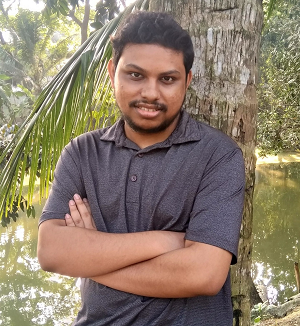
\includegraphics[width=2.8cm]{images/photo.png}
}
\end{tabularx}
\begin{center}
\begin{tabularx}{\linewidth}{@{}*{2}{X}@{}}
% left side %
{
    \csection{ABOUT ME}{\small
\justify
I would like to introduce myself as a technology enthusiast who always likes to work with the latest technologies. I also study and keep me updated about the latest technology gadgets. Being an aspiring computer science student, I always try to bring out the best in myself. Though my primary interests include Computer Security and Web Development, I also like to solve programming problems regularly on various online judges.}
\vspace{0.5cm}
    
    \csection{EDUCATION}{\small
        \begin{itemize}
            % item 1 %
            \item \frcontent{B.Sc. in Computer Science and Engineering}{Shahjalal University of Science and Technology}{}{2016-2021}
            \item \frcontent{Higher Secondary School Certificate}{Chittagong Urea Fertilizer College}{GPA: 5.00}{2016}
        \end{itemize}
    }
    \csection{SKILLS}{\small
        \begin{itemize}
            \item \textbf{Tools \& Technologies} \newline
            {\footnotesize C, C++, Java, Python, Javascript, HTML, CSS, Java Swing, MySQL, Laravel, Android Studio, Wordpress, Git and Github, Linux}{}{}
            \item \textbf{Industry Knowledge} \newline
            {\footnotesize Object Oriented Programming, Data Structures, Machine Learning, Web Development, Search Engine Optimization, Teamwork}
        \end{itemize}
    }
    \csection{SOCIAL LINKS}{
    \vspace{0.3cm}
    \faGithub \hspace{0.2cm}\clink{\href{https://github.com/Nirzak}{https://github.com/Nirzak}}
    
    \faLinkedin \hspace{0.2cm}\clink{\href{https://linkedin.com/in/Nirzak}{https://linkedin.com/in/Nirzak}}
    }
} 
% end left side %
& 
% right side %
{
    \csection{PROJECTS}{\small
        \begin{itemize}
            \item \frcontent{EncryptDecrypt \clink{\href{https://github.com/Nirzak/EncryptDecrypt}{[github.com/Nirzak/EncryptDecrypt]}}}{A simple software to Encrypt and Decrypt any file or text}{}{Java, Java Swing}
            \item \frcontent{Crime-Reporting-App \clink{\href{https://github.com/Nirzak/Crime-Reporting-App}{[github.com/Nirzak/Crime-Reporting-App]}}}{An android app to report nearby crime incidents with many more features.}{}{Java}
            \item \frcontent{ProjectCatalogger \clink{\href{https://github.com/Nirzak/Project-Catalogger}{[github.com/Nirzak/Project-Catalogger]}}}{A website to catalog all student projects in one directory}{}{HTML, PHP, MySQL, Laravel}
            \item \frcontent{Self-Forwarder-Bot \clink{\href{https://github.com/Nirzak/Self-Forwarder-Bot}{[github.com/Nirzak/Self-Forwarder-Bot]}}}{A telegram bot to forward own files to send them anonymously}{}{Python}
            \item \frcontent{PhishDetector \clink{\href{https://github.com/Nirzak/PhishDetector}{[github.com/Nirzak/PhishDetectort]}}}{A chrome extension to detect phishing sites using machine learning model}{}{Javascript, Python}
        \end{itemize}
    }
    \csection{HOBBIES \& INTERESTS}{\small
        \vspace{0.32cm}
        \begin{tabularx}{\linewidth}{@{}*{4}{>{\centering\arraybackslash}X}@{}}
            {\centering
            
\includegraphics[width=0.8cm]{images/music.png}
            } &
            {\centering
            
\includegraphics[width=0.8cm]{images/lamp.png}
            } & 
            {\centering
            
\includegraphics[width=0.8cm]{images/shield.png}
            } &
            {\centering
            
\includegraphics[width=0.8cm]{images/cauldron.png}
            } \\
            {\footnotesize Music} & {\footnotesize Problem Solving} & {\footnotesize Cyber Security} & {\footnotesize Open Source}
        \end{tabularx}
    }
}
\end{tabularx}
\end{center}
\end{document}